% Threshold ECDSA + Trustless DKG Integration into TLS 1.3
% Combined Proposal + Handshake Workflow
\documentclass[11pt]{article}
\usepackage[a4paper,margin=1in]{geometry}
\usepackage{hyperref}
\usepackage{amsmath, amssymb}
\usepackage{booktabs}
\usepackage{longtable}
\usepackage{tabularx}
\usepackage{enumitem}
\usepackage{xcolor}
\usepackage{listings}
\usepackage{graphicx}
\usepackage{caption}
\usepackage{fancyhdr}
\usepackage{tikz}
\usetikzlibrary{positioning,arrows.meta,shapes.geometric}
\usepackage{inconsolata}
\usepackage{svg}
\usepackage{array}
\usepackage{setspace}
\setstretch{1.05}

\hypersetup{colorlinks=true,linkcolor=blue,urlcolor=blue,citecolor=purple}
\pagestyle{fancy}
\fancyhf{}
\lhead{Threshold ECDSA for TLS 1.3}
\rhead{Proposal + Workflow}
\cfoot{\thepage}

% Code listing style
\lstdefinestyle{code}{
  basicstyle=\ttfamily\small,
  backgroundcolor=\color{gray!10},
  frame=single,
  breaklines=true,
  showstringspaces=false,
  keywordstyle=\color{blue!70!black},
  commentstyle=\color{green!40!black},
  stringstyle=\color{orange!50!black}
}
\lstset{style=code}

\newcolumntype{Y}{>{\raggedright\arraybackslash}X}
\newcommand{\sectionline}{\vspace{0.5em}\hrule\vspace{0.8em}}

\title{Integrating Fast Multiparty Threshold ECDSA with Fast Trustless Setup into TLS 1.3}
\author{Internal Security Engineering Draft}
\date{November 2025}

\begin{document}
\maketitle
\tableofcontents
\sectionline

\section{Executive Summary}
This document combines a comprehensive proposal and detailed handshake workflow for integrating a modern Fast Multiparty Threshold ECDSA scheme together with a trustless Distributed Key Generation (DKG) protocol into existing TLS~1.3 infrastructure without altering wire semantics. The integration decentralizes private key control, limits blast radius of node compromise, preserves client transparency, and maintains low-latency server authentication.

\subsection{What is Threshold Cryptography?}
\textbf{Threshold cryptography} is a cryptographic primitive that distributes trust among multiple parties. Instead of a single entity holding a complete private key, the key is split into multiple \textit{shares} distributed across $N$ participants. Any subset of $T$ participants (the \textit{threshold}) can cooperate to perform cryptographic operations (e.g., signing), but fewer than $T$ participants learn nothing about the private key.

\paragraph{Key Properties:}
\begin{itemize}[leftmargin=*]
  \item \textbf{Secret Sharing:} Private key $x$ never exists in one location; instead, shares $x_1, x_2, \ldots, x_N$ are distributed such that $x$ can be reconstructed (implicitly, not explicitly) only with $\ge T$ shares.
  \item \textbf{Threshold Signing:} To sign message $m$, at least $T$ parties contribute partial signatures $\sigma_i$; these are combined into a standard signature $\sigma$ verifiable with the public key.
  \item \textbf{Robustness:} Compromise of up to $T-1$ parties reveals no information about the key; the system remains secure.
  \item \textbf{Availability:} As long as $\ge T$ honest participants are online, operations proceed normally.
\end{itemize}

\paragraph{Why Threshold ECDSA for TLS?}
Traditional TLS deployments store private keys in single locations (servers, HSMs). If compromised, attackers can impersonate servers indefinitely. Threshold ECDSA eliminates this single point of failure: an attacker must compromise $\ge T$ geographically and administratively separated nodes simultaneously—a significantly harder attack. Moreover, the scheme is \textit{transparent to clients}: standard TLS handshakes proceed unchanged; clients verify signatures using the same public key as before.

\paragraph{Trustless Setup (DKG):}
Traditional secret sharing requires a trusted dealer to split the key. A \textit{Distributed Key Generation (DKG)} protocol allows participants to jointly generate a keypair without any party ever knowing the full private key, eliminating the dealer as a point of trust or failure.

\begin{figure}[h]
\centering
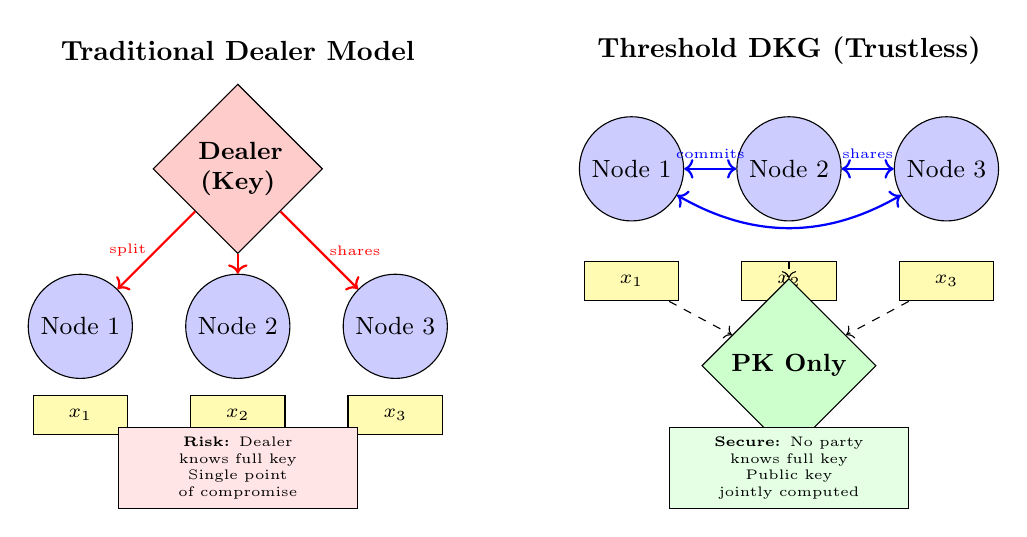
\begin{tikzpicture}[
  node distance=0.3cm,
  signer/.style={draw, circle, minimum size=1.3cm, fill=blue!20, font=\small},
  share/.style={draw, rectangle, minimum width=1.2cm, minimum height=0.5cm, fill=yellow!30, font=\scriptsize},
  key/.style={draw, diamond, minimum size=1.2cm, fill=red!20, font=\small\bfseries}
]

% Traditional (Dealer Model)
\node[font=\bfseries] at (-3, 2.5) {Traditional Dealer Model};
\node[key] (dealer) at (-3, 1) {\parbox{1cm}{\centering Dealer\\(Key)}};
\node[signer] (t1) at (-5, -1) {Node 1};
\node[signer] (t2) at (-3, -1) {Node 2};
\node[signer] (t3) at (-1, -1) {Node 3};
\node[share, below=0.2cm of t1] (sh1) {$x_1$};
\node[share, below=0.2cm of t2] (sh2) {$x_2$};
\node[share, below=0.2cm of t3] (sh3) {$x_3$};

\draw[->, thick, red] (dealer) -- (t1) node[midway, left, font=\tiny] {split};
\draw[->, thick, red] (dealer) -- (t2);
\draw[->, thick, red] (dealer) -- (t3) node[midway, right, font=\tiny] {shares};

\node[draw, rectangle, fill=red!10, text width=2.8cm, font=\tiny, align=center] at (-3, -2.8) {
  \textbf{Risk:} Dealer knows full key\\
  Single point of compromise
};

% Threshold DKG Model
\node[font=\bfseries] at (4, 2.5) {Threshold DKG (Trustless)};
\node[signer] (d1) at (2, 1) {Node 1};
\node[signer] (d2) at (4, 1) {Node 2};
\node[signer] (d3) at (6, 1) {Node 3};

\draw[<->, thick, blue] (d1) -- (d2) node[midway, above, font=\tiny] {commits};
\draw[<->, thick, blue] (d2) -- (d3) node[midway, above, font=\tiny] {shares};
\draw[<->, thick, blue] (d1) to[bend right=30] (d3);

\node[share, below=0.5cm of d1] (dsh1) {$x_1$};
\node[share, below=0.5cm of d2] (dsh2) {$x_2$};
\node[share, below=0.5cm of d3] (dsh3) {$x_3$};

\node[key, fill=green!20] (pubkey) at (4, -1.5) {PK Only};
\draw[->, dashed] (dsh1) -- (pubkey);
\draw[->, dashed] (dsh2) -- (pubkey);
\draw[->, dashed] (dsh3) -- (pubkey);

\node[draw, rectangle, fill=green!10, text width=2.8cm, font=\tiny, align=center] at (4, -2.8) {
  \textbf{Secure:} No party knows full key\\
  Public key jointly computed
};

\end{tikzpicture}
\caption{Comparison of traditional dealer-based secret sharing vs. trustless Distributed Key Generation (DKG). In DKG, participants exchange commitments and shares via multi-party computation; the private key is never materialized.}
\end{figure}

\section{Objectives}
\begin{itemize}[leftmargin=*]
  \item Threshold-protect server certificate keys: public key retained, private key never reconstructed.
  \item Trustless (dealerless) key setup with robustness against up to $f$ malicious/Byzantine participants.
  \item Zero client modifications; RFC~8446 compliance.
  \item Added signing latency median $<10$ ms; strong auditability and rotation workflows.
  \item Scalable precomputation for high throughput (hundreds of handshakes per second).
\end{itemize}

\section{Scope and Non-Goals}
\textbf{In Scope:} Server cert thresholdization, optional internal threshold CA, TLS CertificateVerify signing, OCSP/SCT support, operational tooling.\\
\textbf{Out of Scope (initial):} Client certificate threshold, PQC threshold primitives, cross-organizational federation.

\section{Stakeholders}
Security Engineering, Platform/Infra, Compliance/Governance, SRE/DevOps, Application Teams.

\section{Background and Motivation}
\subsection{The Problem with Centralized Private Keys}
Traditional TLS deployments rely on a single private key stored on the server or in a Hardware Security Module (HSM). While HSMs provide tamper resistance, they remain \textit{logical single points of failure}:
\begin{itemize}[leftmargin=*]
  \item \textbf{Key Exfiltration:} If compromised (firmware exploit, supply chain attack, insider threat), the attacker obtains the complete key.
  \item \textbf{Impersonation Risk:} A stolen key allows indefinite server impersonation until certificate revocation propagates.
  \item \textbf{Limited Blast Radius Control:} HSM compromise affects all certificates sharing that key.
  \item \textbf{Operational Rigidity:} Key rotation requires certificate reissuance and careful propagation windows.
\end{itemize}

\subsection{Threshold Cryptography as a Solution}
Threshold ECDSA disperses key material across $N$ geographically and administratively separated nodes. A quorum of $T$ nodes collaborates to produce signatures, but fewer than $T$ reveals \textit{nothing} about the private key. Benefits include:
\begin{itemize}[leftmargin=*]
  \item \textbf{Defense in Depth:} Attacker must compromise $\ge T$ nodes simultaneously across different security domains.
  \item \textbf{Graceful Degradation:} Up to $N-T$ nodes can fail or be taken offline without service disruption.
  \item \textbf{Auditability:} Every signature involves multiple parties; logs provide multi-party attestation.
  \item \textbf{Proactive Security:} Share refresh protocols allow re-randomizing shares periodically, mitigating slow key leakage.
\end{itemize}

\subsection{Fast Variants and Trustless Setup}
Modern schemes (Lindell--Nof, Gennaro--Goldfeder) achieve:
\begin{itemize}[leftmargin=*]
  \item \textbf{Two-round signing} with aggressive precomputation of ephemeral nonces, enabling latencies competitive with local HSM operations ($<10$ ms added).
  \item \textbf{Trustless DKG} eliminating the dealer: participants jointly generate the keypair via multi-party computation without any party learning the full key.
\end{itemize}
These advances make threshold ECDSA practical for high-throughput, latency-sensitive deployments like TLS servers at scale.

\section{Requirements}
\subsection{Functional}
\begin{itemize}[leftmargin=*]
  \item Distributed key generation for curve P-256 (primary) or secp256k1 (optional) with configurable $(N,T)$.
  \item Produce valid ECDSA $(r,s)$ signatures for TLS CertificateVerify.
  \item Proactive share refresh without altering public key.
  \item High availability: tolerate $<T$ offline nodes.
\end{itemize}
\subsection{Security}
\begin{itemize}[leftmargin=*]
  \item Unforgeability under threshold ECDSA assumptions.
  \item Confidential share storage; hardened memory; encrypted rest state.
  \item Audit trail: transcript hash, quorum identity, aggregated $R$.
  \item Nonce safety; bias resistance; misbehavior detection and eviction.
\end{itemize}
\subsection{Performance}
Median added latency $\le 10$ ms; $p99 \le 25$ ms. Horizontal scaling via precompute workers.\\
\subsection{Operational}
Automated health, rotation workflow, disaster recovery with threshold backups.

\section{Threat Model}
Adversaries: external attackers, insiders, network interceptors, malicious signer nodes. Goals: prevent key reconstruction with $<T$ shares, prevent nonce reuse, detect rogue-key attempts, maintain attribution.

\section{Architecture Overview}
\subsection{Components}
Signer Nodes (share custody)\; Coordinator (orchestration)\; Auditor Service\; Precomputation Workers\; PKI Integration Layer\; Monitoring Stack.

\subsection{Data Flow Summary}
\begin{enumerate}[leftmargin=*]
  \item \textbf{DKG:} Broadcast commitments and shares; derive public key $Q$.
  \item \textbf{Precompute:} Generate nonce tuples $(k_i, R_i)$ and auxiliary inversion data.
  \item \textbf{Signing:} Aggregate $R = \sum R_i$, derive $r$, compute partial $s_i$, aggregate $s$.
  \item \textbf{TLS Frontend:} Consumes $(r,s)$ as if locally generated.
\end{enumerate}

\section{Cryptographic Protocol Details}
\subsection{Distributed Key Generation}
Each party selects polynomial $f_i$ of degree $T-1$; share for party $p$ is $s_p = \sum_i f_i(p)$. Commitments (Pedersen/Feldman) ensure verifiability; abort on inconsistency. Public key $Q = (\sum_i f_i(0))G$.
\subsection{Precomputation}
Signers compute pools of nonces $k_i$ and points $R_i = k_i G$ with auxiliary values for fast inversion. Coordinator tracks availability.
\subsection{Signing}
Given transcript hash $m$, each signer returns partial $s_i = k_i^{-1}(m + r x_i)$ (scheme variant dependent). Final $s = \sum s_i \mod n$, low-$s$ normalization applied.
\subsection{Share Refresh}
Proactive refresh via secondary polynomials randomizes shares; $Q$ unchanged.
\subsection{Misbehavior Detection}
Invalid partials trigger blame protocols requiring commitment proofs; malicious nodes quarantined.

\section{TLS 1.3 Integration Points}
The threshold signing mechanism integrates seamlessly into TLS 1.3 by substituting only the \textit{CertificateVerify} ECDSA signing operation. All other protocol steps remain unchanged:

\begin{itemize}[leftmargin=*]
  \item \textbf{Certificate Message:} Contains the public key $Q$ derived from the threshold DKG. Clients use this public key for standard ECDSA verification.
  \item \textbf{CertificateVerify Signature:} Instead of using a local private key, the TLS frontend (via OpenSSL 3 provider or PKCS\#11 engine) invokes the threshold signing coordinator with the transcript hash $TH_1$. The coordinator orchestrates partial signature collection and aggregation, returning a standard ECDSA $(r,s)$ pair.
  \item \textbf{Session Tickets:} Unaffected (symmetric key encryption).
  \item \textbf{OCSP Responses, SCTs, CRL Signing:} Can reuse the same threshold signing path if the issuing key is also threshold-protected.
  \item \textbf{Client Perspective:} Completely transparent. The client performs standard RFC 8446 handshake verification; no knowledge of or changes required for threshold backend.
\end{itemize}

\paragraph{Implementation Hook:}
The OpenSSL 3 Provider API allows custom signing backends. The threshold provider intercepts \texttt{EVP\_PKEY\_sign} calls, marshals the digest to the coordinator, awaits the threshold signature, and returns it as if computed locally. Fallback mechanisms handle quorum unavailability gracefully (e.g., retry, alert, or optional secondary conventional key per policy).

\section{Operational Workflow}
\subsection{Lifecycle Phases}
\begin{enumerate}[leftmargin=*]
  \item \textbf{Bootstrap (DKG):} Deploy signer nodes with ephemeral bootstrap identities; run distributed key generation protocol; each node stores its share $x_i$ encrypted at rest; public key $Q$ published and certificate issued by CA.
  \item \textbf{Normal Signing:} TLS frontend requests signatures for incoming handshakes; coordinator selects $T$ healthy signers; partials aggregated; $(r,s)$ returned.
  \item \textbf{Precompute Pool Maintenance:} Background workers on signer nodes generate nonce tuples $(k_i, R_i)$ and register with coordinator; pool size monitored (target: e.g., 1000 tuples); autoscaling triggered if depletion risk detected.
  \item \textbf{Key Rotation:} Run parallel DKG for new keypair $Q'$; issue certificate for $Q'$; dual-publish both certificates during transition window; after propagation (e.g., 48h), deprecate old $Q$; archive logs and securely erase old shares.
  \item \textbf{Proactive Refresh:} Periodic (e.g., weekly) share refresh via polynomial re-sharing; $Q$ unchanged but shares $x_i$ randomized, mitigating long-term partial leakage accumulation.
  \item \textbf{Incident Response:} If node compromise suspected, exclude from quorum; run emergency refresh or expedited rotation; forensic audit of signing logs.
  \item \textbf{Decommission:} Securely wipe share storage; revoke node membership; update coordinator configuration; verify no residual key material.
\end{enumerate}

\section{High Availability}
Example: $N=7, T=4$. Latency-aware quorum selection; fallback policy on insufficient quorum; optional secondary conventional key (policy-gated).

\section{Performance Considerations}
Intra-DC RTT (2--3 ms) + partial compute (<2 ms) + aggregation (<1 ms) yields target median 5--8 ms. Parallel precompute amortizes expensive inversions.

\section{API Contract (Draft)}
\begin{lstlisting}[language=json,caption={Signing API Request/Response}]
POST /v1/sign
{ "hash": "<hex>", "context": "TLS-1.3-CertificateVerify", "nonce_policy": "fresh" }

Response:
{ "r": "<hex>", "s": "<hex>", "pubkey": "<hex>",
  "quorum": ["S1","S3","S5","S6"],
  "precompute_id": "uuid", "timestamp": "2025-11-13T12:34:56Z" }
\end{lstlisting}
Errors: 409 QuorumInsufficient, 424 PrecomputeDepleted, 400 InvalidHashFormat, 500 InternalAggregationError.

\section{Logging and Audit}
Append-only log (Kafka or similar) with hashing chain; daily Merkle root published for transparency.

\section{Security Analysis Summary}
\begin{itemize}[leftmargin=*]
  \item Share Theft (<$T$): No reconstruction.
  \item Nonce Bias: Verifiable commitments; single-use enforcement.
  \item Rogue-Key: Commitment + ZK proof checks.
  \item DoS by Malicious Signer: Adaptive quorum; eviction.
  \item Coordinator Compromise: No forging without shares.
\end{itemize}

\section{Testing and Validation}
Unit (arithmetic invariants), integration (local cluster handshake), fuzzing (commitment/partial corruption), chaos (mid-round node termination), performance benchmarks, timing side-channel probes, compliance mapping.

\section{Implementation Phases}
\begin{center}
\begin{tabular}{|l|c|l|}
\hline
Phase & Duration & Deliverables \\
\hline
0 Research & 2 wks & Protocol selection, curve finalization \\
1 Prototype & 4 wks & Minimal cluster, REST API, tests \\
2 TLS Integration & 3 wks & OpenSSL provider, handshake demo \\
3 Hardening & 4 wks & Audit log, refresh, fault tolerance \\
4 Rotation \& CA & 3 wks & Key rotation flow, threshold CA (opt.) \\
5 Production Rollout & 4 wks & Monitoring, DR plan, docs \\
\hline
\end{tabular}
\end{center}

\section{Risk and Mitigation}
\begin{center}
\begin{tabular}{|p{3.2cm}|p{2.4cm}|p{6.2cm}|}
\hline
Risk & Impact & Mitigation \\
\hline
Protocol Complexity Bugs & Invalid/forgeable signatures & Use vetted libraries; formal verification of arithmetic core \\
Latency Spikes & Handshake slowdown & Precompute pools; autoscale; SLO alerts \\
Coordinator Bottleneck & Throughput cap & Stateless multi-instance; idempotent requests \\
Share Leakage Over Time & Gradual compromise & Weekly proactive refresh; hardened memory handling \\
Malicious Node Abort Storm & Availability degradation & Blame protocol; eviction; rapid replacement provisioning \\
Operational Misconfig & Downtime/security gap & IaC validation; canary deployment; config policy checks \\
\hline
\end{tabular}
\end{center}

\section{Future Extensions}
Client-side threshold auth, PQC threshold (Dilithium/FROST-like EdDSA), multi-cloud distribution, transparency log publication, confidential computing enclaves.

\section{Compliance and Governance}
Documented DKG ceremony, RBAC for maintenance, audited break-glass processes, periodic third-party review.

\section{Deployment Model}
Kubernetes: Signer nodes as StatefulSets (AZ anti-affinity), coordinators as Deployments with HPA, Vault/Sealed Secrets for share sealing.

\section{Open Questions}
Threshold parameters $(N,T)$; curve choice (performance vs acceptance); library selection vs custom implementation; inclusion timing for threshold CA; audit publication cadence.

\section{Acceptance Criteria}
Valid TLS handshake to unmodified client with threshold-generated signature meeting latency SLO; successful share refresh without key change; simulated $<T$ compromise fails to reconstruct key; zero-downtime rotation observed over 24h.

\section{Summary}
Decentralizing TLS private keys via fast threshold ECDSA materially reduces compromise risk while preserving protocol compatibility and performance. Structured phased rollout mitigates complexity and ensures auditability.

% -------------------------------------------------------------
\section{Detailed TLS 1.3 Handshake Workflow (Threshold Integration)}
\subsection{Legend}
C: Client; FE: TLS Frontend; COORD: Coordinator; $S_i$: Signer node; PK: Public key; PrePool: Precomputed nonce pool.

\subsection{Pre-Handshake Preparation}
DKG completion, membership list, precompute pool fill, health checks, secure authenticated channels.

\subsection{Standard Phases}
ClientHello; ServerHello; EncryptedExtensions; Certificate; \textbf{CertificateVerify (threshold signing)}; Finished; Application Data.

\subsection{Happy Path Step-by-Step}
\begin{enumerate}[leftmargin=*]
  \item C $\to$ FE: ClientHello.
  \item FE selects cipher suite / group; returns ServerHello.
  \item Key schedule derivation (HKDF) by FE.
  \item FE sends EncryptedExtensions.
  \item FE sends Certificate containing PK.
  \item Transcript hash $TH_1$ computed.
  \item FE submits threshold SignRequest($TH_1$) to COORD.
  \item COORD selects quorum $Q$ of size $T$ with available precompute tuples.
  \item COORD instructs each signer to participate using chosen tuple.
  \item Each signer computes partial $(R_i, s_i)$ and returns with proof.
  \item COORD aggregates $R=\sum R_i$, derives $r$, verifies partials, computes $s=\sum s_i$ (normalizes low-$s$).
  \item COORD returns final $(r,s)$ to FE.
  \item FE sends CertificateVerify with $(r,s)$.
  \item FE sends Finished.
  \item Client verifies signature (standard ECDSA over transcript) and sends Finished.
  \item Secure channel established; application data flows.
\end{enumerate}

\subsection{Failure Paths}
\paragraph{Insufficient Quorum:} Error returned; FE retries/backoff or policy fallback.\\
\paragraph{Precompute Depletion:} Refill triggered; request retried post replenishment.\\
\paragraph{Invalid Partial:} Blame protocol; malicious node evicted; round restarted.\\
\paragraph{Coordinator Failure:} FE resubmits idempotent request to alternate coordinator.\\
\paragraph{Client Abort:} Consumed nonces discarded to avoid reuse.

\subsection{Security Checks During Signing}
Nonce single-use enforcement; low-$s$ normalization; transcript hash validation; audit logging (request id, quorum, aggregated $R$ hash).

\subsection{Complete TLS 1.3 Handshake with Threshold Signing (Illustrated)}
\begin{figure}[h]
\centering
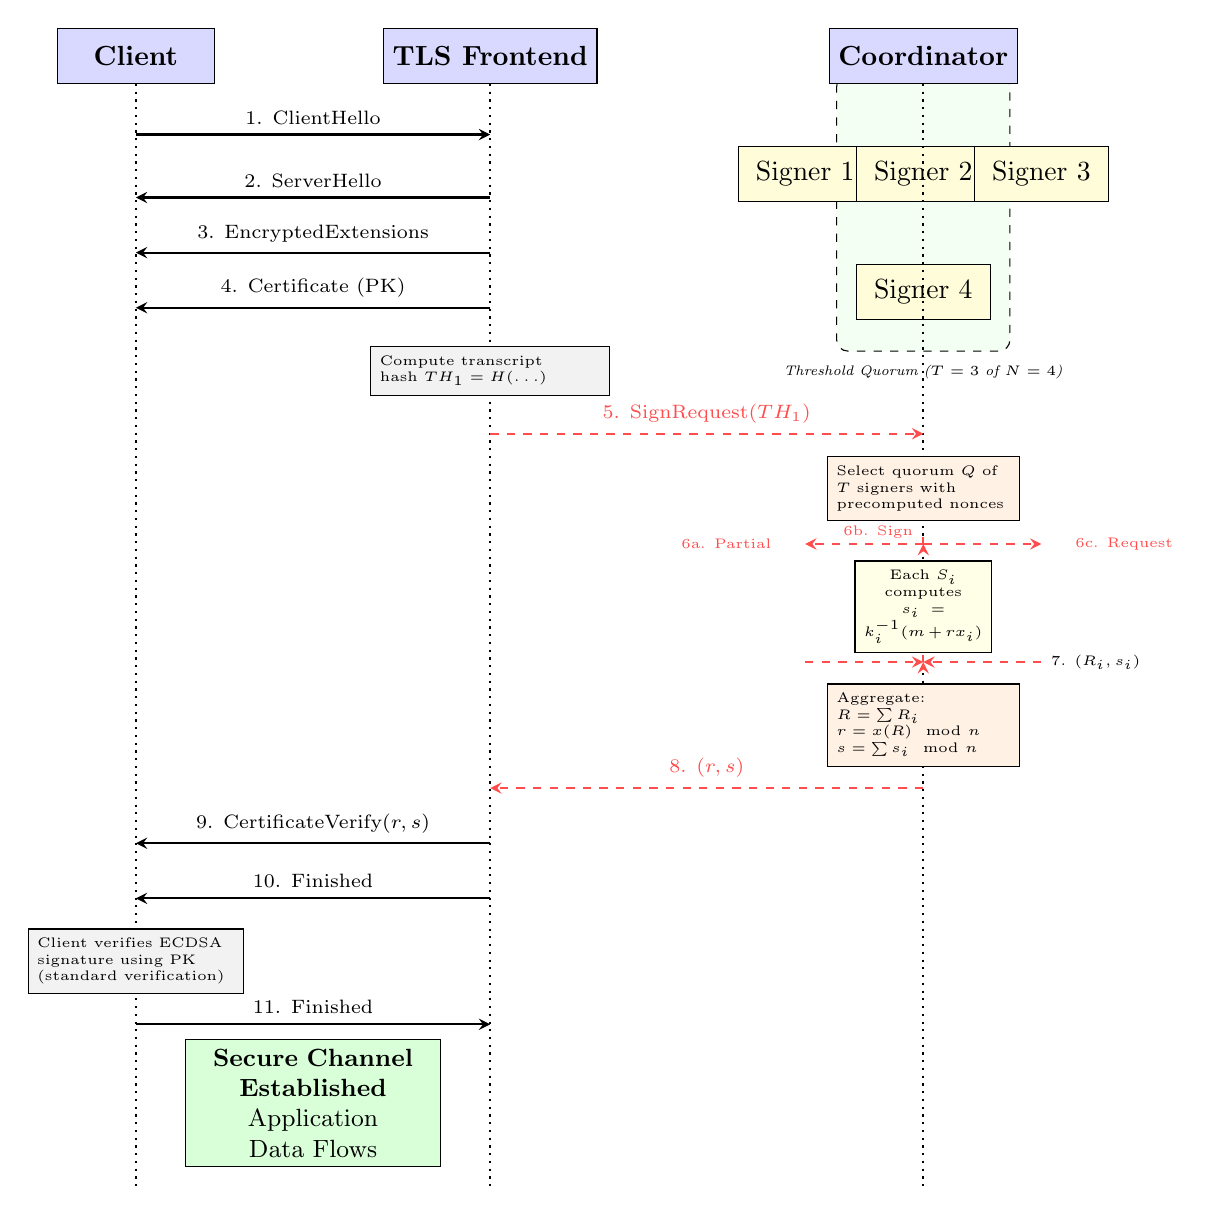
\begin{tikzpicture}[
  >=stealth,
  node distance=0.4cm,
  actor/.style={draw, rectangle, minimum width=2cm, minimum height=0.7cm, fill=blue!15},
  message/.style={->, thick},
  internal/.style={->, thick, dashed, red!70},
  group/.style={draw, rectangle, rounded corners, dashed, fill=green!5, minimum width=2.2cm}
]

% Actors
\node[actor] (client) at (0,0) {\textbf{Client}};
\node[actor] (frontend) at (4.5,0) {\textbf{TLS Frontend}};
\node[group, minimum height=3.5cm] (siggroup) at (10,-2) {};
\node[actor] (coord) at (10,0) {\textbf{Coordinator}};
\node[actor, fill=yellow!15, minimum width=1.7cm] (s1) at (8.5,-1.5) {Signer 1};
\node[actor, fill=yellow!15, minimum width=1.7cm] (s2) at (10,-1.5) {Signer 2};
\node[actor, fill=yellow!15, minimum width=1.7cm] (s3) at (11.5,-1.5) {Signer 3};
\node[actor, fill=yellow!15, minimum width=1.7cm] (s4) at (10,-3) {Signer 4};
\node[below=0.05cm of siggroup, font=\tiny\it] {Threshold Quorum ($T=3$ of $N=4$)};

% Vertical lines
\draw[dotted, thick] (client.south) -- ++(0,-14);
\draw[dotted, thick] (frontend.south) -- ++(0,-14);
\draw[dotted, thick] (coord.south) -- ++(0,-14);

% Messages
\coordinate (c1) at (0,-1);
\coordinate (f1) at (4.5,-1);
\draw[message] (c1) -- (f1) node[midway, above, font=\scriptsize] {1. ClientHello};

\coordinate (f2) at (4.5,-1.8);
\coordinate (c2) at (0,-1.8);
\draw[message] (f2) -- (c2) node[midway, above, font=\scriptsize] {2. ServerHello};

\coordinate (f3) at (4.5,-2.5);
\coordinate (c3) at (0,-2.5);
\draw[message] (f3) -- (c3) node[midway, above, font=\scriptsize] {3. EncryptedExtensions};

\coordinate (f4) at (4.5,-3.2);
\coordinate (c4) at (0,-3.2);
\draw[message] (f4) -- (c4) node[midway, above, font=\scriptsize] {4. Certificate (PK)};

% Internal note
\node[draw, rectangle, fill=gray!10, text width=2.8cm, font=\tiny, align=left] (note1) at (4.5,-4) {
  Compute transcript\\
  hash $TH_1 = H(\ldots)$
};

% Threshold signing sequence
\coordinate (f5) at (4.5,-4.8);
\coordinate (co1) at (10,-4.8);
\draw[internal] (f5) -- (co1) node[midway, above, font=\scriptsize] {5. SignRequest($TH_1$)};

\node[draw, rectangle, fill=orange!10, text width=2.2cm, font=\tiny, align=left] (note2) at (10,-5.5) {
  Select quorum $Q$ of\\
  $T$ signers with\\
  precomputed nonces
};

\coordinate (co2) at (10,-6.2);
\coordinate (s1a) at (8.5,-6.2);
\coordinate (s2a) at (10,-6.2);
\coordinate (s3a) at (11.5,-6.2);
\draw[internal] (co2) -- (s1a) node[left, font=\tiny, xshift=-0.3cm] {6a. Partial};
\draw[internal] (co2) -- (s2a) node[left, font=\tiny, yshift=0.15cm] {6b. Sign};
\draw[internal] (co2) -- (s3a) node[right, font=\tiny, xshift=0.3cm] {6c. Request};

\node[draw, rectangle, fill=yellow!10, text width=1.5cm, font=\tiny, align=center] (note3) at (10,-7) {
  Each $S_i$ computes\\
  $s_i = k_i^{-1}(m + rx_i)$
};

\coordinate (s1b) at (8.5,-7.7);
\coordinate (s2b) at (10,-7.7);
\coordinate (s3b) at (11.5,-7.7);
\coordinate (co3) at (10,-7.7);
\draw[internal] (s1b) -- (co3);
\draw[internal] (s2b) -- (co3);
\draw[internal] (s3b) -- (co3);
\node[right, font=\tiny] at (11.5,-7.7) {7. $(R_i, s_i)$};

\node[draw, rectangle, fill=orange!10, text width=2.2cm, font=\tiny, align=left] (note4) at (10,-8.5) {
  Aggregate:\\
  $R = \sum R_i$\\
  $r = x(R) \mod n$\\
  $s = \sum s_i \mod n$
};

\coordinate (co4) at (10,-9.3);
\coordinate (f6) at (4.5,-9.3);
\draw[internal] (co4) -- (f6) node[midway, above, font=\scriptsize] {8. $(r,s)$};

\coordinate (f7) at (4.5,-10);
\coordinate (c5) at (0,-10);
\draw[message] (f7) -- (c5) node[midway, above, font=\scriptsize] {9. CertificateVerify$(r,s)$};

\coordinate (f8) at (4.5,-10.7);
\coordinate (c6) at (0,-10.7);
\draw[message] (f8) -- (c6) node[midway, above, font=\scriptsize] {10. Finished};

\node[draw, rectangle, fill=gray!10, text width=2.5cm, font=\tiny, align=left] (note5) at (0,-11.5) {
  Client verifies ECDSA\\
  signature using PK\\
  (standard verification)
};

\coordinate (c7) at (0,-12.3);
\coordinate (f9) at (4.5,-12.3);
\draw[message] (c7) -- (f9) node[midway, above, font=\scriptsize] {11. Finished};

\node[draw, rectangle, fill=green!15, text width=3cm, font=\small, align=center] (final) at (2.25,-13.3) {
  \textbf{Secure Channel Established}\\
  Application Data Flows
};

\end{tikzpicture}
\caption{Complete TLS 1.3 handshake with threshold ECDSA signing integration. Steps 5--8 (red dashed) represent the threshold signing subprotocol invoked during CertificateVerify generation. Client remains unaware of the distributed signing process.}
\end{figure}

\subsection{Latency Budget (Illustrative)}
\begin{center}
\begin{tabular}{|l|c|}
\hline Component & Time (ms) \\
\hline FE $\to$ COORD Dispatch & 0.3 \\
Fan-out to Signers & 0.5 \\
Partial Compute (parallel) & 1.5 \\
Aggregate \& Verify & 0.7 \\
Return to FE & 0.3 \\
\hline Total Added (median) & $\approx 3.3$ \\
\hline
\end{tabular}
\end{center}

\subsection{Monitoring Metrics}
\begin{itemize}[leftmargin=*]
  \item \texttt{tls\_threshold\_sign\_duration\_ms} (Histogram): End-to-end signing latency distribution.
  \item \texttt{tls\_threshold\_quorum\_size} (Gauge): Number of signers participating per request.
  \item \texttt{tls\_threshold\_precompute\_pool\_depth} (Gauge): Available nonce tuples per signer.
  \item \texttt{tls\_threshold\_abort\_count} (Counter): Failed signing attempts (timeout, invalid partial).
  \item \texttt{tls\_threshold\_malicious\_flagged} (Counter): Nodes flagged by blame protocol.
  \item \texttt{tls\_threshold\_requests\_total} (Counter): Total signing requests received.
  \item \texttt{tls\_threshold\_coordinator\_queue\_depth} (Gauge): Pending requests at coordinator.
\end{itemize}

\section{References}
\begin{itemize}[leftmargin=*]
  \item RFC 8446: TLS 1.3.
  \item Lindell, Nof (2021): Fast Secure Two-Party ECDSA.
  \item Gennaro, Goldfeder (2018): Fast Multiparty Threshold ECDSA.
  \item SEC 1: Elliptic Curve Cryptography.
  \item OpenSSL Provider API Docs.
  \item FROST Draft: Round-Optimized Schnorr Threshold Signatures.
\end{itemize}

\end{document}
